\subsubsection{Conceptual Models}\label{sec_conceptual}

This section focuses on descriptions from primary sources that \progname{} is
based on, included for transparency to ensure a direct connection to the
original material. The $13$ models are grouped by concern:
\begin{enumerate}

    \item Emotion structure and types [\cref{C_Emotion},
    \cref{C_EmotionStruct}, \cref{C_ComplexEmotion},
    \cref{C_ComplexEmotions-CTE}, \cref{C_PAD}]

    \item Emotion generation, intensity, and decay [\cref{C_Appraisal-CTE},
    \cref{C_EmOther}, \cref{C_EmIntensity-CTE}, \cref{C_EmDecay}]

    \item Knowledge necessary for generating emotion via PES and CTE
    [\cref{C_Goals}, \cref{C_Plans}, \cref{C_Attention}, \cref{C_Relation-CTE}]

\end{enumerate}

~\newline\noindent
\begin{minipage}{\textwidth}
    \renewcommand*{\arraystretch}{1.5}
    \begin{tabular}{| p{\colAwidth}  p{\colBwidth}|}
        \hline
        \rowcolor[gray]{0.9}
        \bf C\refstepcounter{conceptnum}\theconceptnum \label{C_Emotion} & \bf
        Emotion \\\hline
    \end{tabular}
\end{minipage}

\paragraph{Description} An emotion is a short-term affective state representing
the coordinated physiological and behavioural response of the brain and body to
events that an organism perceives as relevant (e.g. it impacts their goals
(\cref{C_Goals})).

Some researchers hypothesize that each emotion has a \textit{signature}
representing the coordinated response pattern it typically causes, including:
behavioural and expressional characteristics; somatic and neurophysiological
factors that prepare the body for action; cognitive and interpretive
evaluations that give rise to the emotion; and experiential and subjective
qualities unique to an individual. Elements of the signature can be innate or
learned.

Emotion is also characterized by its high intensity relative to other types of
affect, its tendency to come and go quickly, its association with a specific
triggering event, object, or person, and clear cognitive contents.

CTE states that emotions do not always require cognition, and they do not have
a internal symbolic structure that is significant to the system (i.e.
non-propositional signals). The signals propagate through the system on a
global level, setting and maintaining the system in a mode (emotion ``mode'').
\\\hrule

\paragraph{Source} \citet[p.~4]{jeon2017emotions},
\citet[p.~138--140]{scherer2000psychological},
\citet[p.~349--350]{broekens2021emotion}, \citet[p.~249]{frijda1986emotions},
\citet[p.~121]{smith2001toward}, \citet[p.~133]{hudlicka2019modeling},
\citet[p.~108]{scherer2001appraisalB}, \citet[p.~6]{carlson1992psychology},
\cite{oatley1987towards}

\paragraph{Depends On} \cref{C_Goals}

\paragraph{Ref. By} \cref{C_EmIntensity-CTE}, \cref{C_EmDecay},
\tyref{TY_EmotionState}, \tyref{TY_Emotion} \\\hrule\vspace{0.5mm}\hrule

~\newline

\noindent
\begin{minipage}{\textwidth}
    \renewcommand*{\arraystretch}{1.5}
    \begin{tabular}{| p{\colAwidth}  p{\colBwidth}|}
        \hline
        \rowcolor[gray]{0.9}
        \bf C\refstepcounter{conceptnum}\theconceptnum \label{C_EmotionStruct}
        &
        \bf Emotion Structure (PES) \\\hline
    \end{tabular}
\end{minipage}

\paragraph{Description} PES organizes its eight emotion kinds---\textit{Fear},
\textit{Anger}, \textit{Sadness}, \textit{Joy}, \textit{Interest},
\textit{Surprise}, \textit{Disgust}, and \textit{Acceptance}---into a cone
(Figure~\ref{fig_emotionsolid}).

The emotion types are arranged on a circular plane based on their relative
similarity as determined from empirically gathered responses. In this way,
emotions considered the most dissimilar appear on opposite sides of the plane.
The vertical axis of the solid represents emotional intensity, with the most
intense emotions at the top and a state of ``deep sleep'' at the bottom point.
The cone shape implies that the differences between the emotions becomes less
distinct at low intensities.

\begin{figure}[H]
    \centering
    \begin{subfigure}[c]{0.55\textwidth}
        \centering

        $\vcenter{\hbox{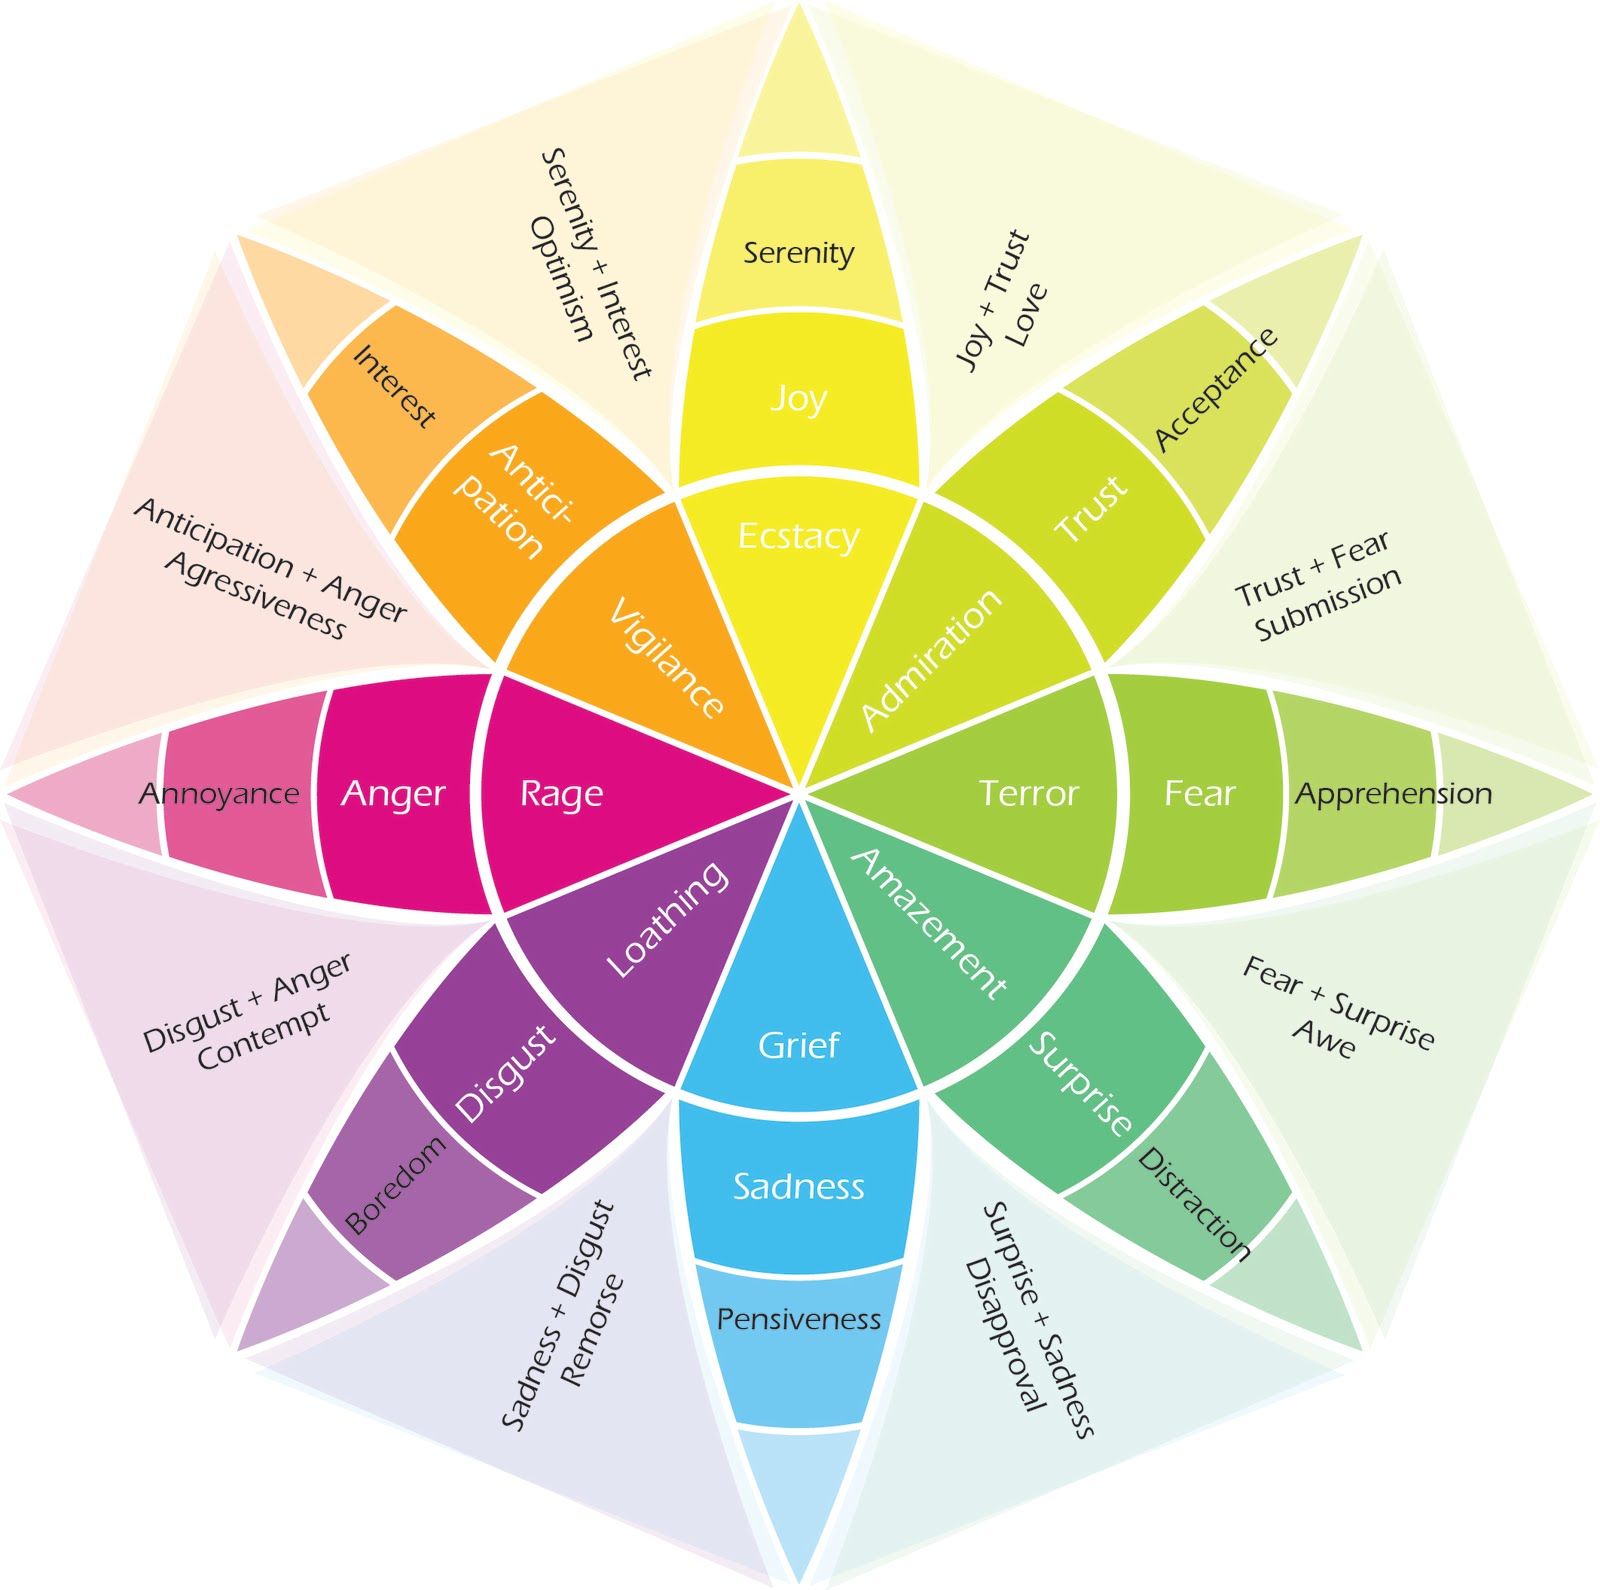
\includegraphics[width=\textwidth]{figures/plutchik_emotion_solid.jpg}}}$
        \label{fig_2d}
    \end{subfigure} \hspace{0.05\textwidth} %
    \begin{subfigure}[c]{0.25\textwidth}
        \centering

        $\vcenter{\hbox{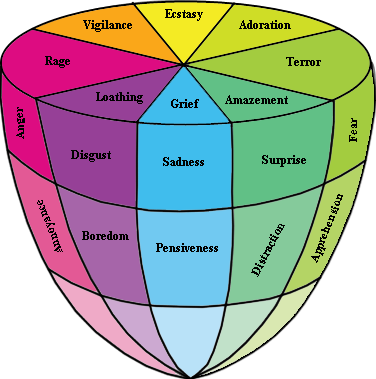
\includegraphics[width=\textwidth]{figures/plutchik_solid.png}}}$
        \label{fig_3d}
    \end{subfigure}
    \caption{A flattened and 3D view of the Emotion Structure}
    \label{fig_emotionsolid}
\end{figure}

\hrule

\paragraph{Source} \cite{robert1980emotion, block1957studies,
conte1976circumplex}

\paragraph{Depends On} --

\paragraph{Ref. By} \cref{C_ComplexEmotion}, \tref{T_GetEmotionStatePAD},
\tyref{TY_EmotionKind} \\\hrule\vspace{0.5mm}\hrule

~\newline

\noindent
\begin{minipage}{\textwidth}
    \renewcommand*{\arraystretch}{1.5}
    \begin{tabular}{| p{\colAwidth}  p{\colBwidth}|}
        \hline
        \rowcolor[gray]{0.9}
        \bf C\refstepcounter{conceptnum}\theconceptnum \label{C_ComplexEmotion}
        &\bf Mixing Emotions (PES) \\\hline
    \end{tabular}
\end{minipage}

\paragraph{Description} PES states that complex emotions are mixtures of
emotion types and intensity. It uses a colour wheel analogy to describe how to
mix them, where Emotion categories are hues and intensity is saturation.

In the PES structural model (\cref{C_EmotionStruct}), the tip of the cone has
no colour saturation whereas the circular plane is fully saturated with colour,
respectively representing no intensity and full intensity.
\\\hrule

\paragraph{Source} \cite{robert1980emotion}

\paragraph{Depends On} \cref{C_EmotionStruct}

\paragraph{Ref. By} \rref{R_MixingEmotionsPES}, \rref{R_PartitionEmotions}
\\\hrule\vspace{0.5mm}\hrule

\newpage\noindent
\begin{minipage}{\textwidth}
    \renewcommand*{\arraystretch}{1.5}
    \begin{tabular}{| p{\colAwidth}  p{\colBwidth}|}
        \hline
        \rowcolor[gray]{0.9}
        \bf C\refstepcounter{conceptnum}\theconceptnum
        \label{C_ComplexEmotions-CTE}
        &\bf ``Complex'' Emotions (CTE) \\\hline
    \end{tabular}
\end{minipage}

\paragraph{Description} CTE proposes that ``complex'' emotions are elaborations
of the emotion ``modes'' (\cref{C_Appraisal-CTE}), where the system ascribes
additional propositional meanings to it. For example, \textit{Disgust} is
typically called \textit{Contempt}, \textit{Disdain}, or \textit{Hatred} when
felt towards people instead of food, toxins, and/or
contamination~\citep[p.~60]{oatley1992best}. This also means that ``[e]motions
are in part socially constructed, but they are constructed around a biological
basis.''~\citep[p.~119]{oatley1992best}

This often requires a ``model of the self'' to draw meaning from, developed via
individual differences and culture. This model is also tied to the individual's
relationships with others (\cref{C_Relation-CTE}). \\\hrule

\paragraph{Source} \cite{oatley1987towards, oatley1992best}

\paragraph{Depends On} \cref{C_Appraisal-CTE}, \cref{C_Relation-CTE}

\paragraph{Ref. By} \tref{T_CalculateEmotionAcceptance},
\rref{R_MixingEmotionsCTE} \\\hrule\vspace{0.5mm}\hrule

~\newline

\noindent
\begin{minipage}{\textwidth}
    \renewcommand*{\arraystretch}{1.5}
    \begin{tabular}{| p{\colAwidth}  p{\colBwidth}|}
        \hline
        \rowcolor[gray]{0.9}
        \bf C\refstepcounter{conceptnum}\theconceptnum
        \label{C_PAD}
        &\bf PAD Space \\\hline
    \end{tabular}
\end{minipage}

\paragraph{Description} Based on studies in a variety of related fields with
the goal of quantifying different types of affective phenomena (e.g. emotion,
core affect, mood, personality), PAD describes describes a small set of nearly
orthogonal dimensions for analysing emotional states and behaviours, while as
relating them to other affect types and experiences. Points in this space can
represent different affective phenomena. The dimensions are present in all
affective reactions that are operative in any situation:
\begin{itemize}
    \item \textit{Pleasure} measures the positive-negative aspects of the
    emotion state (related to \textit{valence}),

    \item \textit{Arousal} is how alert and active the individual is in that
    state, and

    \item \textit{Dominance} is how much control the individual feels they have
    in that state.
\end{itemize}

The range of each dimension is $-1$ to $1$ representing mean ratings for
emotion terms. Means are based on ratings from $16$ to $31$ subjects,
transformed to the $-1$ to $1$ scale. Statistical significance---measured from
a mean of $0$---and standard deviations differ between ratings.

Three dimensions are optimal for general characterizations and measurements of
emotional states, as two dimensions cannot distinguish between clusters of
affect and additional dimensions added little value to evaluations\\\hrule

\paragraph{Source} \cite{mehrabian1980basic, mehrabian1996pleasure}

\paragraph{Depends On} --

\paragraph{Ref. By} \tref{T_GetEmotionStatePAD}, \tyref{TY_PAD}
\\\hrule\vspace{0.5mm}\hrule

~\newpage

\noindent
\begin{minipage}{\textwidth}
    \renewcommand*{\arraystretch}{1.5}
    \begin{tabular}{| p{\colAwidth}  p{\colBwidth}|}
        \hline
        \rowcolor[gray]{0.9}
        \bf C\refstepcounter{conceptnum}\theconceptnum \label{C_Appraisal-CTE}
        &\bf Emotion Modes (CTE) \\\hline
    \end{tabular}
\end{minipage}

\paragraph{Description} CTE hypothesises that a system can change its emotion
``mode'' (i.e. type) at plan junctures, identifiable by changes in the likely
success of a plan (\cref{C_Plans}). These junctures are assumed to be
distinctive and recurring. The system enters a ``mode'' based on the current
plan state and if/how goals (\cref{C_Goals}) are impacted, and form the basis
for other emotion ``types'' (see \cref{C_ComplexEmotions-CTE}).

\begin{table}[H]
    \centering
    \label{tab:cte_pattern}
    \renewcommand{\arraystretch}{1.2}
    \begin{tabular}{lll}
        \toprule
        \textbf{Emotion} & \textbf{Juncture of Current Plan} & \textbf{Next
        State} \\ \midrule

        \rowcolor[gray]{0.9}\textit{Happiness} & Sub-goals being achieved &
        Continue, modifying if needed \\

        \textit{Sadness} & Failure of a major plan or loss of an active goal &
        Do nothing/Search for a new plan \\

        \rowcolor[gray]{0.9}\textit{Anxiety} & Self-preservation goal
        threatened & Stop, Attend to Environment/Escape \\

        \textit{Anger} & Active plan frustrated & Try harder/Aggress \\

        \rowcolor[gray]{0.9}\textit{Disgust} & Gustatory goal violated & Reject
        substance/Withdraw \\

        \bottomrule
    \end{tabular}
\end{table}

CTE proposes that the emotion ``modes'' inhibit each other, and there might
also be conflicts that prevent the system from settling into a ``mode''. Being
in an emotion ``mode'' is a necessary---but not sufficient---condition to
experience emotion. A true emotion also requires the assignment of meaning to
the ``mode'' and the scheduling of voluntary actions. \\\hrule

\paragraph{Source} \cite{oatley1987towards, oatley1992best}

\paragraph{Depends On} \cref{C_Goals}, \cref{C_Plans}

\paragraph{Ref. By} \cref{C_ComplexEmotions-CTE}, \cref{C_EmOther},
\cref{C_EmIntensity-CTE}, \tref{T_CalculateEmotionGP}
\\\hrule\vspace{0.5mm}\hrule

~\newline

\noindent
\begin{minipage}{\textwidth}
    \renewcommand*{\arraystretch}{1.5}
    \begin{tabular}{| p{\colAwidth}  p{\colBwidth}|}
        \hline
        \rowcolor[gray]{0.9}
        \bf  C\refstepcounter{conceptnum}\theconceptnum \label{C_EmOther} & \bf
        ``Other Emotions''\\ \hline
    \end{tabular}
\end{minipage}

\paragraph{Description} Researchers continue to debate if \textit{Surprise} and
\textit{Interest} are ``emotions''. CTE is unsure of their status, but proposes
that:
\begin{itemize}
    \item Sudden, unexpected events cause \textit{Surprise}, and could
    represent an interruption and abrupt transition to another emotion ``mode''
    (\cref{C_Appraisal-CTE})

    \item Sustained attention (\cref{C_Attention}) to certain external events
    implies \textit{Interest}
\end{itemize}

Both descriptions imply that \textit{Surprise} and \textit{Interest} can
coexist with, or are part of, other emotion ``modes''.\\\hrule

\paragraph{Source} \cite{oatley1987towards, oatley1992best}

\paragraph{Depends On} \cref{C_Appraisal-CTE}, \cref{C_Attention}

\paragraph{Ref. By} \tref{T_CalculateEmotionSurprise},
\tref{T_CalculateEmotionInterest}
\\\hrule\vspace{0.5mm}\hrule

~\newline

\noindent
\begin{minipage}{\textwidth}
    \renewcommand*{\arraystretch}{1.5}
    \begin{tabular}{| p{\colAwidth}  p{\colBwidth}|}
        \hline
        \rowcolor[gray]{0.9}
        \bf C\refstepcounter{conceptnum}\theconceptnum
        \label{C_EmIntensity-CTE}
        &\bf Emotion Intensity (CTE) \\\hline
    \end{tabular}
\end{minipage}

\paragraph{Description} Overall, emotion intensity is a relatively understudied
topic. CTE proposes that the intensity of an emotion (\cref{C_Emotion})
corresponds to how entrained the system is in a ``mode''
(\cref{C_Appraisal-CTE}) and to what degree it is ``locked into'' it. \\\hrule

\paragraph{Source} \cite{frijda1992complexity, oatley1987towards,
oatley1992best}

\paragraph{Depends On} \cref{C_Emotion}, \cref{C_Appraisal-CTE}

\paragraph{Ref. By} \tref{T_CalculateEmotionIntensity}
\\\hrule\vspace{0.5mm}\hrule

~\newline

\noindent
\begin{minipage}{\textwidth}
    \renewcommand*{\arraystretch}{1.5}
    \begin{tabular}{| p{\colAwidth}  p{\colBwidth}|}
        \hline
        \rowcolor[gray]{0.9}
        \bf  C\refstepcounter{conceptnum}\theconceptnum \label{C_EmDecay} & \bf
        Emotion Decay\\ \hline
    \end{tabular}
\end{minipage}

\paragraph{Description} Emotions (\cref{C_Emotion}) do not last
indefinitely---they dissipate after a time, implying the presence of an emotion
decay mechanism. This requires a specification of baseline values for each
emotion and as well as one or more decay functions. \\\hrule

\paragraph{Source} \cite{broekens2021emotion}

\paragraph{Depends On} \cref{C_Emotion}

\paragraph{Ref. By} \tref{T_DecayEmotionState} \\\hrule\vspace{0.5mm}\hrule

~\newline

\noindent
\begin{minipage}{\textwidth}
    \renewcommand*{\arraystretch}{1.5}
    \begin{tabular}{| p{\colAwidth}  p{\colBwidth}|}
        \hline
        \rowcolor[gray]{0.9}
        \bf C\refstepcounter{conceptnum}\theconceptnum \label{C_Goals} & \bf
        Goals \\\hline
    \end{tabular}
\end{minipage}

\paragraph{Description} Goals compel systems to act in ways that achieve a
desired objective. They are essential for emotion processing, identifying
what elements of the current world state are relevant to an individual rather
than relying on properties of the environment alone. Goals are also connected
to emotions, partially motivating emotion-driven behaviours.

PES describes goals as being in service to global adaptational problems,
whereas CTE view them as symbolic representations of possible environmental
states that a system wants to achieve. \\\hrule

\paragraph{Source} \cite{oxfordGoals}, \citet[p.~223]{broekens2016emotional},
\cite{robert1980emotion, oatley1987towards}

\paragraph{Depends On} --

\paragraph{Ref. By} \cref{C_Emotion}, \cref{C_Appraisal-CTE}, \cref{C_Plans},
\tref{T_CalculateEmotionGP}, \tyref{TY_Goal} \\\hrule\vspace{0.5mm}\hrule

~\newline

\noindent
\begin{minipage}{\textwidth}
    \renewcommand*{\arraystretch}{1.5}
    \begin{tabular}{| p{\colAwidth}  p{\colBwidth}|}
        \hline
        \rowcolor[gray]{0.9}
        \bf C\refstepcounter{conceptnum}\theconceptnum \label{C_Plans} & \bf
        Plans (CTE) \\\hline
    \end{tabular}
\end{minipage}

\paragraph{Description} CTE describes plans as sequences of transformations
between symbolic representations of possible environmental states, linking the
current state to a goal (\cref{C_Goals}). To ``make'' a plan is to create a
sequence of transformations, and to ``execute'' the plan is to enact the
sequence in the world.

A system forms plans with imperfect and incomplete knowledge of the
environment, and often only looks one or two steps ahead. \\\hrule

\paragraph{Source} \cite{oatley1987towards}

\paragraph{Depends On} \cref{C_Goals}

\paragraph{Ref. By} \cref{C_Appraisal-CTE}, \tref{T_CalculateEmotionGP},
\tyref{TY_Plan} \\\hrule\vspace{0.5mm}\hrule

~\newline

\noindent
\begin{minipage}{\textwidth}
    \renewcommand*{\arraystretch}{1.5}
    \begin{tabular}{| p{\colAwidth}  p{\colBwidth}|}
        \hline
        \rowcolor[gray]{0.9}
        \bf C\refstepcounter{conceptnum}\theconceptnum \label{C_Attention} &
        \bf Attention \\\hline
    \end{tabular}
\end{minipage}

\paragraph{Description} Attention is a set of mechanisms that allow a
limited-capacity system to select salient or goal-relevant information. These
mechanisms might work in parallel. Behavioural effects of attention vary
between systems, partially due to personality. \\\hrule

\paragraph{Source} \cite{oxfordAttention}

\paragraph{Depends On} --

\paragraph{Ref. By} \cref{C_EmOther}, \tyref{TY_Attention}
\\\hrule\vspace{0.5mm}\hrule

~\newline

\noindent
\begin{minipage}{\textwidth}
    \renewcommand*{\arraystretch}{1.5}
    \begin{tabular}{| p{\colAwidth}  p{\colBwidth}|}
        \hline
        \rowcolor[gray]{0.9}
        \bf C\refstepcounter{conceptnum}\theconceptnum \label{C_Relation-CTE} &
        \bf Social Relationship \\\hline
    \end{tabular}
\end{minipage}

\paragraph{Description} CTE states that many emotions are social, occurring in
the course of one's relationships with others. This allows them to construct
mutual plans to coordinate the actions of multiple actors, which also requires
each actor to have a ``model of the self''.

The emotion of \textit{Acceptance} (i.e. \textit{Trust})---an elementary
component of social life---in PES also implies the existence of relationships
with others. ``Affective trust'' builds on past experiences with, feelings of
security, confidence, and satisfaction towards, and the perceived level of
selfless concern demonstrated by a partner regardless of what the future holds.
The biological basis of affective trust might lie in social attachment and
affiliation due to the role of oxytocin.

A social relationship is a representation of the history shared between the
individual and another person, entity, or thing. They can be established
implicitly based on precedents and customs (i.e. culture). \\\hrule

\paragraph{Source} \cite{oatley1987towards, oxfordTrust, rempel1985trust}

\paragraph{Depends On} --

\paragraph{Ref. By} \cref{C_ComplexEmotions-CTE},
\tref{T_CalculateEmotionAcceptance}, \tyref{TY_Relation-CTE}
\\\hrule\vspace{0.5mm}\hrule